\documentclass{article}
\usepackage[left=3cm, right=3cm, top=2cm]{geometry} 
\usepackage[utf8]{inputenc}
\usepackage{hyphenat}
\usepackage{mathdesign}
\usepackage{verbatim}
\usepackage{float}
\renewcommand{\thesubsection}{\arabic{subsection}}
\title{Efficient Matrix Multiplication}
\author{Garg, Poorva\\
    \texttt{poorva98@gmail.com}
    \and
    Senthilnathan, Aditya\\
    \texttt{aditsep99@gmail.com}}
\date{February 2019}

\usepackage{natbib}
\usepackage{graphicx}

\begin{document}

\maketitle

\section*{Objective of the Assignment}
Taking convolution of two matrices can be done very efficiently if we employ matrix multiplication which itself is a very expensive thing to do in terms of execution time. So, beside the brute force algorithm, we tried 3 different techniques to make matrix multiplication efficient - used linear algebra libraries like mkl and openBlas, used multithreading in c++. Analyzing the outcomes of these new codes was the objective of this assignment

\section*{Commands for Different Matrix Multiplication Algorithms}
To compile the code, run following commands on terminal\\
\texttt{\$ export LD\_LIBRARY\_PATH=/path\_to\_your\_openblas\_installation\_directory/lib/}\\
\texttt{\$ export MKLROOT=/path\_to\_your\_mkl\_installation\_directory/intel/mkl/}\\
\texttt{\$ make}\\
\\
To delete the compiled code\\
\texttt{\$ make clean}\\
\\
To use convolution employing different matrix multiplications, below are the instructions:
\begin{enumerate}
    \item To use brute force algorithm\\
    \texttt{\$ ./output.out convolve\_with\_padding input\_matrix.txt number\_of\_rows\_of\_input\_matrix \\matrix2.txt number\_of\_rows\_of\_kernel}\\
    \texttt{\$ ./output.out convolve\_without\_padding input\_matrix.txt number\_of\_rows\_of\_input\_matrix matrix2.txt number\_of\_rows\_of\_kernel}
    
    \item To use MKL Library\\
    \texttt{\$ ./output.out convolve\_with\_padding\_matrixmult\_with\_mkl input\_matrix.txt\\ number\_of\_rows\_of\_input\_matrix matrix2.txt number\_of\_rows\_of\_kernel}\\
    \texttt{\$ ./output.out convolve\_without\_padding\_matrixmult\_with\_mkl input\_matrix.txt\\ number\_of\_rows\_of\_input\_matrix matrix2.txt number\_of\_rows\_of\_kernel}\\
    
    \item To use OpenBlas Library\\
    \texttt{\$ ./output.out convolve\_with\_padding\_matrixmult\_with\_openblas input\_matrix.txt\\ number\_of\_rows\_of\_input\_matrix matrix2.txt number\_of\_rows\_of\_kernel}\\
    \texttt{\$ ./output.out convolve\_without\_padding\_matrixmult\_with\_openblas input\_matrix.txt\\ number\_of\_rows\_of\_input\_matrix matrix2.txt number\_of\_rows\_of\_kernel}\\
    
    \item To use multithreading\\
    \texttt{\$ ./output.out convolve\_with\_padding\_matrixmult\_with\_pthreads input\_matrix.txt\\ number\_of\_rows\_of\_input\_matrix matrix2.txt number\_of\_rows\_of\_kernel}\\
    \texttt{\$ ./output.out convolve\_without\_padding\_matrixmult\_with\_pthreads input\_matrix.txt\\ number\_of\_rows\_of\_input\_matrix matrix2.txt number\_of\_rows\_of\_kernel}\\
    
\end{enumerate}

\section*{Linear Algebra Libraries}
Let us first describe the two linear algebra libraries which perform the matrix multiplication with utmost efficiency
\subsection*{Intel\textsuperscript{\textregistered} MKL Library}
Intel\textsuperscript{\textregistered} Math Kernel Library \cite{mkl} is a computing math library of highly optimized, extensively threaded routines for applications that require maximum performance. The library provides Fortran and C programming language interfaces. Intel MKL C language interfaces can be called from applications written in either C or C++, as well as in any other language that can reference a C interface.

\subsection*{OpenBLAS Library}
OpenBLAS \cite{openBLAS} is an optimized BLAS library based on GotoBLAS2 1.13 BSD version. In scientific computing, OpenBLAS is an open source implementation of the BLAS (Basic Linear Algebra Subprograms) API with many hand-crafted optimizations for specific processor types. It is developed at the Lab of Parallel Software and Computational Science, ISCAS. OpenBLAS adds optimized implementations of linear algebra kernels for several processor architectures, including Intel Sandy Bridge and Loongson. It claims to achieve performance comparable to the Intel MKL.

\section*{Performance Comparison of MKL and OpenBLAS}
We implemented matrix multiplication using linear algebra libraries MKL and OpenBLAS and recorded the execution time they take in two different situations
\subsection{Multiple Execution on Same Size Matrices}
We ran our code to multiply matrices of 50X50 500 times and collected the data of execution time taken to find mean and standard deviation and found that both the libraries give similar performance on small sized matrices.\\
\begin{center}
\begin{tabular}[h]{|l|l|l|l|l|}
\hline
\multicolumn{3}{|c|}{Data of 500 times execution} \\
\hline
Data & MKL & OpenBLAS\\
\hline
Mean & 0.00019351 & 0.00019351\\
\hline
Standard Deviation & 5.9966E-05 & 5.6906E-05\\
\hline
\end{tabular}
\end{center}



\subsection{Executing Once on Different Size Matrices}
We ran our code to multiply matrices of various sizes ranging from size 1X1 to 300X300 and collected the data of execution time taken to find mean and standard deviation and found that both the libraries give similar performance. But since this time, large sized matrices were also there, MKL emerged out to perform slightly better.\\
\begin{center}
\begin{tabular}[h]{|l|l|l|l|l|}
\hline
\multicolumn{3}{|c|}{Data of execution on different sized matrices} \\
\hline
Data & MKL & OpenBLAS\\
\hline
Mean & 2.79E-03 & 3.98E-03\\
\hline
Standard Deviation & 0.00235683 & 0.00354337\\
\hline
\end{tabular}
\end{center}

\begin{figure}[h]
\centering
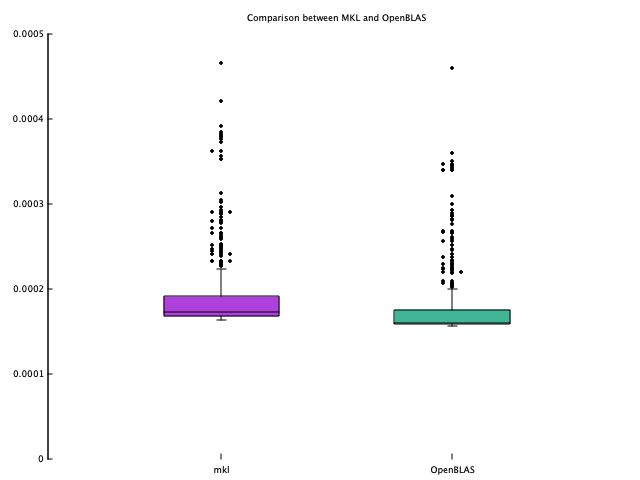
\includegraphics[scale=0.4]{1.png}
\caption{Comparison between MKL and OpenBLAS for same sized matrices}
\label{fig:1.png}
\end{figure}

\begin{figure}[h]
\centering
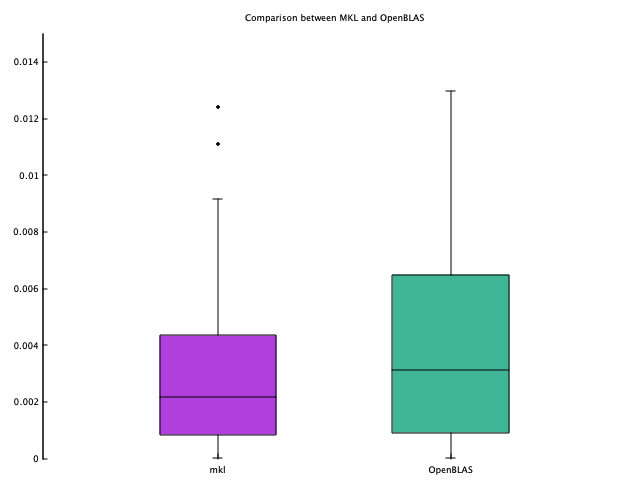
\includegraphics[scale=0.4]{2.png}
\caption{Comparison between MKL and OpenBLAS on Different sized matrices}
\label{fig:2.png}
\end{figure}

\section*{Multithreading with Pthreads}
MKL and OpenBLAS use threading routines to make matrix multiplication efficient. We tried multithreading ourselves to improve the performance of our brute force algorithm. Since our machine had only two cores and only two threads could be run per core, we initiated four threads. We divided our matrix into four parts and multiplied each part separately to the latter matrix to get the final output. Following data of mean and standard deviation and graphs tell us about the performance of our pThreads implementation.\\
\\
It is clearly visible that pThreads implementation was able to perform better than brute force implementation due to division of labour. Though, in case of small sized matrices, the overhead of creting a thread may sometimes, cause it to take more time in execution.
\\
\begin{center}
\begin{tabular}[h!]{|l|l|l|l|l|}
\hline
\multicolumn{3}{|c|}{Data of execution on same sized matrices} \\
\hline
Data & Brute Force & pThreads\\
\hline
Mean & 0.00364517 & 0.00252567\\
\hline
Standard Deviation & 0.00085551 & 0.00064802\\
\hline
\end{tabular}
\end{center}
\begin{center}
\begin{tabular}[h]{|l|l|l|l|l|}
\hline
\multicolumn{3}{|c|}{Data of execution on different sized matrices} \\
\hline
Data & Brute Force & pThreads\\
\hline
Mean & 2.03E-01 & 1.84E-01\\
\hline
Standard Deviation & 0.206982321 & 0.18303028\\
\hline
\end{tabular}
\end{center}

\begin{figure}[h!]
\centering
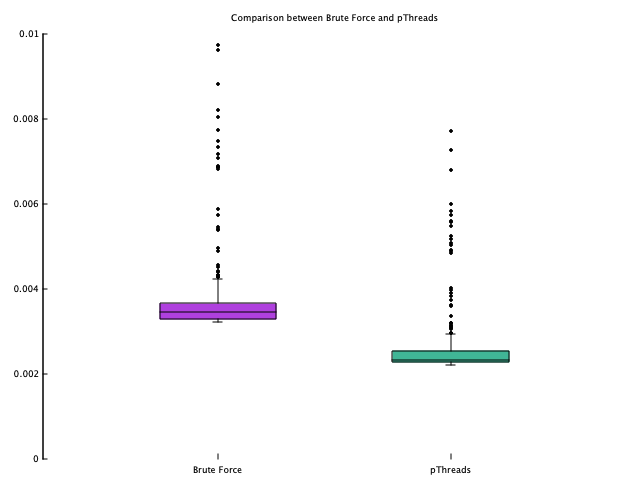
\includegraphics[scale=0.4]{3.png}
\caption{Comparison between Brute Force and pThreads on same sized matrices}
\label{fig:3.png}
\end{figure}

\begin{figure}[h]
\centering
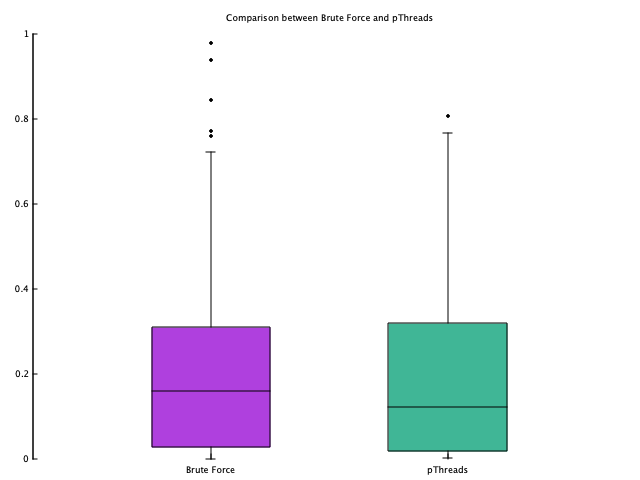
\includegraphics[scale=0.4]{4.png}
\caption{Comparison between Brute Force and pThreads on different sized matrices}
\label{fig:4.png}
\end{figure}

\section*{Image Processing Library and LeNet Architecture}
Along with carefully analyzing the various implementations for matrix multiplication, we also used them to implement our convolution function. We also coded some other image processing functions which include sigmoid, softmax, tanh, relu, maxpool and average pool and further used these functions to implement LeNet architecture to identify digits from MNIST images.\\
\\
In the terminal, go to the directory which contains all the files, and then run following commands to run the code\\
\texttt{\$ python preprocess.py image.png}
\\\texttt{\$ make}
\\\texttt{\$ ./output.out}
\\
\\
To delete the compiled code, run\\
\texttt{\$ make clean}

\bibliographystyle{plain}
\bibliography{main}
\end{document}